% Figure from MATH 556 notes, section 24. Compile with the notes preamble.
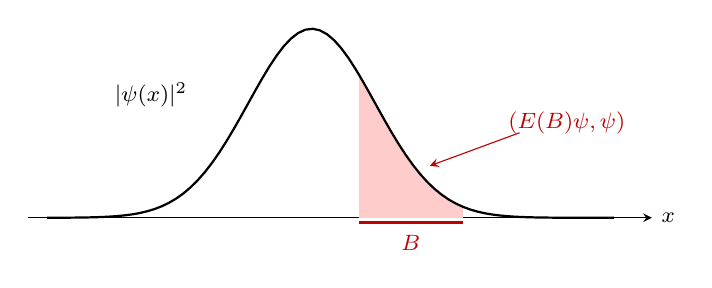
\begin{tikzpicture}[scale=1.2, >=stealth]
    \draw[->] (-3.2,0) -- (3.4,0) node[right, font=\footnotesize] {$x$};
    \fill[red!20, domain=0.3:1.4, samples=40] (0.3,0) -- plot (\x, {2*exp(-(\x+0.2)*(\x+0.2)/0.9)}) -- (1.4,0) -- cycle;
    \draw[thick, domain=-3:3, samples=80] plot (\x, {2*exp(-(\x+0.2)*(\x+0.2)/0.9)});
    \node[font=\footnotesize] at (-1.9,1.3) {$|\psi(x)|^2$};
    \draw[thick, red!75!black] (0.3,-0.05) -- (1.4,-0.05);
    \node[below, font=\footnotesize, red!75!black] at (0.85,-0.08) {$B$};
    \node[font=\footnotesize, red!75!black] at (2.5,1.0) {$(E(B)\psi, \psi)$};
    \draw[->, thin, red!75!black] (2.0,0.9) -- (1.05,0.55);
\end{tikzpicture}
